\documentclass[multi=page,10pt,border={10pt  5pt 5pt 5pt}]{standalone}

\usepackage{graphicx}
\usepackage{helvet}
\usepackage{psfrag}

\renewcommand{\familydefault}{\sfdefault}


\begin{document}

\psfrag{x}{$x$}
\psfrag{y}[rb]{$y$}
\psfrag{N}[rb]{$N$}
\psfrag{dis}[B]{Discretized 2D domain}
\psfrag{quad}[B]{Shape function in Q4 element}
\psfrag{Nquad}[t]{as product of 1D shape functions}
\begin{page}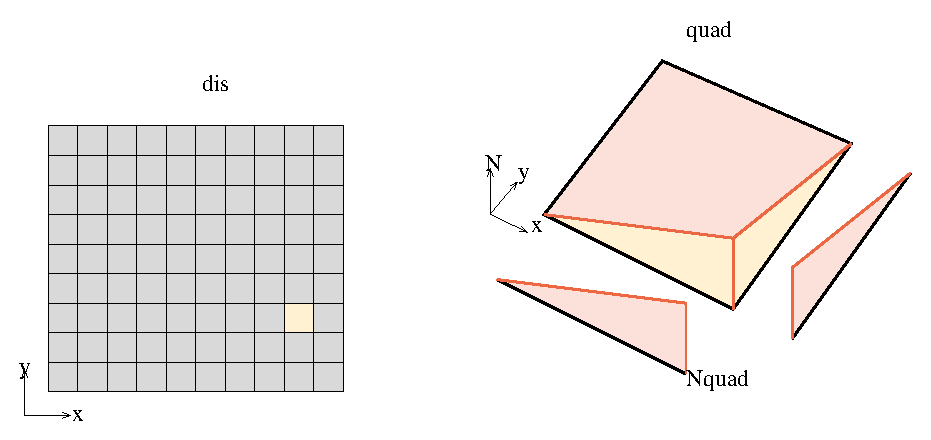
\includegraphics[scale=1.0]{quadFuncs1}\end{page}
\begin{page}
\psfrag{quad}[B]{Nodes of Q9 element}
\psfrag{Nquad}[t]{with quadratic 1D shape functions}
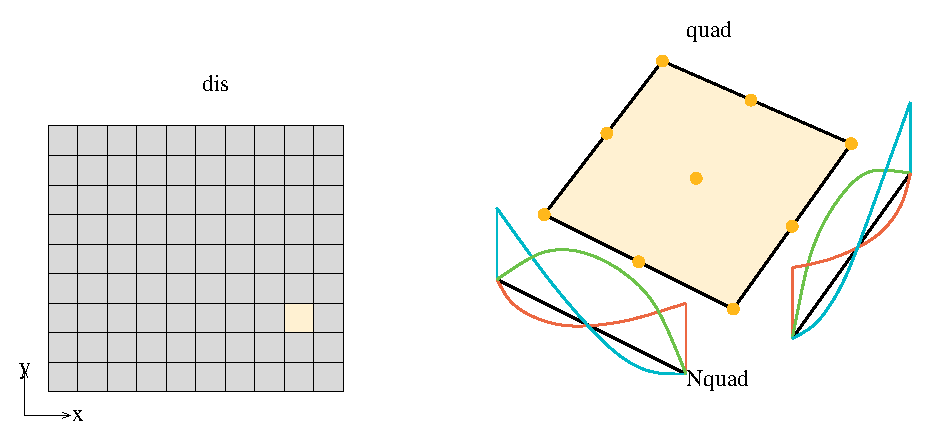
\includegraphics[scale=1.0]{quadFuncs2}\end{page}

\end{document}
